\begin{tframe}{Explaining adversarial examples}

In many application, the precision of an individual input feature is limited [1].

\vspace{0.1in}

Thus, given an input $ x $ and an adversarial input $ \tilde{x} = x + \eta $, a classifier will be expected to assign the same class to both $x$ and $\tilde{x}$ so long as $ \parallel \eta \parallel_\infty < \epsilon $, where $\epsilon$ is smaller than the precision of an individual input feature, so that it will be discarded.

\vspace{0.1in}

Consider the dot product between a weight vector $w$ and an adversarial example $\tilde{x}$:
$$ w^{T}\tilde{x} = w^{T}x + w^{T}\eta $$
The adversarial perturbation causes the activation to grow linearly by $w^{T}\eta$ with the dimension of $w$. This means that for high dimensionality problems, infinitesimal changes to the input add up to one large change to the output.

\end{tframe}

%%--------------------------------------------%%

\begin{tframe}{Generating adversarial examples}

Let $\theta$ be the parameters of a model, x the input to the model, y the targets associated with x (for machine learning tasks that have targets) and $J(\theta, x, y)$ be the cost used to train the neural network. 
We can linearize the cost function around the current value of $\theta$, obtaining an optimal max-norm constrained pertubation of ,

$$ \eta = \epsilon * sign(\nabla_x J(\theta, x, y)) $$

The adversarial examples can thus be obtained as follow,

$$ x = x + \eta $$

In the implementation, $ \epsilon $ is set to 0.1.

\end{tframe}


\begin{tframe}{Generating adversarial examples}

\vspace{0.1in}
\vspace{0.1in}
\vspace{0.1in}

\begin{figure}
  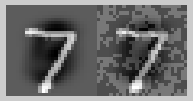
\includegraphics[width=0.4\textwidth]{img/clean-adv.png}
  \caption{Example of adversarial generation.}
\end{figure}

\end{tframe}